\begin{savequote}[75mm] 
Quality is never an accident; it is always the result of intelligent effort. 
\qauthor{John Ruskin.} 
\end{savequote}


\chapter{UT test beam analysis - measurement of the charge sharing
in planar silicon sensors}
\label{chapter:testbeam}

This chapter is dedicated to provides a description of the testbeam studies performed on prototypes of silicon microstrip sensors that will build the Upstream Tracker. The chapter starts by presenting the software that was implemented by the author, which allows performing full data processing. The second part reviews the analysis of charge sharing. 





\section{Timepix3 telescope}
The essential tool that allows making a number of silicon sensor performance studies is TimePix3 telescope, presented in figure \ref{fig:telescope}. 


\begin{figure}[!h]
\centering
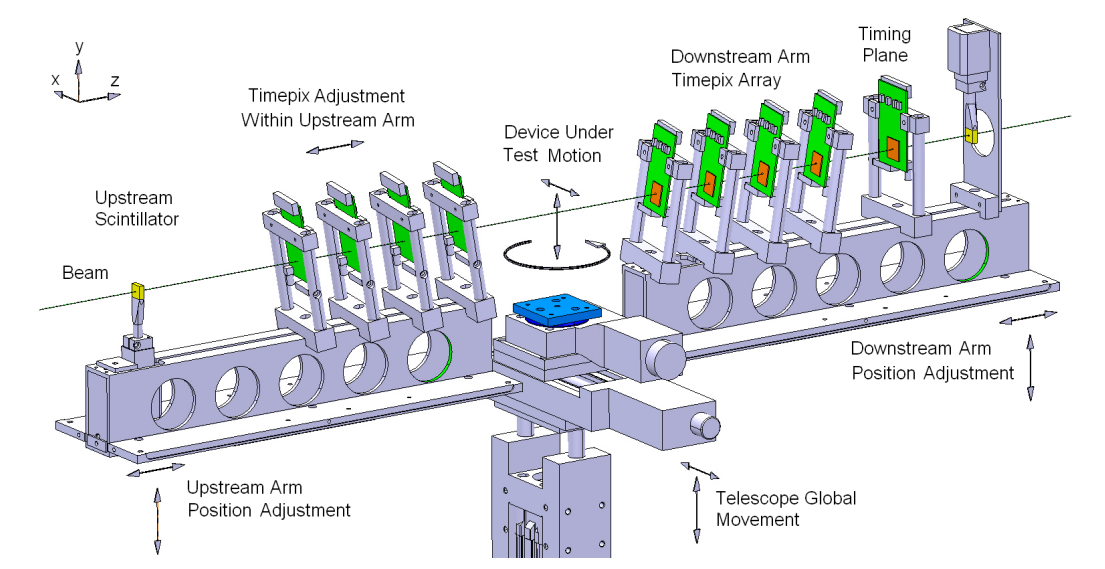
\includegraphics{figures/telescope.png}
\caption{Layout of the Timepix Telescope mechanics, pixel planes and scintillators with respect to the beam axis. Figure taken from \cite{telescope}}
\label{fig:telescope}
\end{figure}


This device consists of 8 plates of 300 µm thick p-on-n sensors bump bonded to the Timepix3 ASIC, divided equally between two arms. The position of each plate along the z-axis is adjustable, typically the distance between each plate is set to be 31 mm, and plates are rotated to an angle of 9 deg in both x and y axis to improve position reconstruction. There is a 200 mm gap between two telescope arms, which is used to place Device Under Test (DUT), see photo \ref{fig:telescope_photo} taken during one of the testbeam companies. The DUT is housed inside a metal box designed to fit into the gap and provides an airtight dry environment cooled via a Peltier device. 
The DUT was installed on a motion stage allowing angular rotations and x and y translations. 

To allow the DUT acquisition trigger two scintillators are placed upstream and downstream of the telescope. The telescope acquisition system doesn't require any trigger signal since it works in a so-called data-driven readout mode in which the data package of each pixel hit is sent immediately after Time-over-Threshold (ToT) conversion. To synchronize DUT clusters with associated Telescope tracks, the information about the trigger timestamp is added to the data recorded by the telescope.  


\begin{figure}[!h]
\centering
\hspace*{-1cm}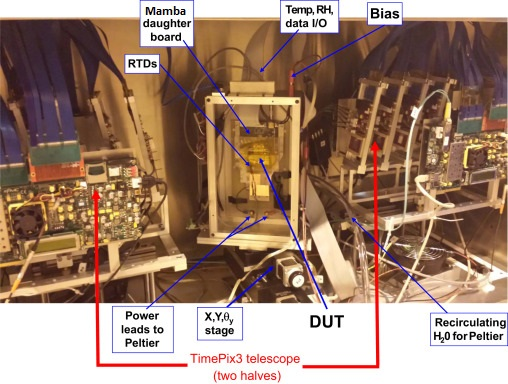
\includegraphics{figures/telescope_photo.jpg}
\caption{The photo of the Timepix Telescope and the DUT inside the box. }
\label{fig:telescope_photo}
\end{figure}

\subsection{TimePix3 Telescope Tracking}

To find the position where the particle interacts with the DUT sensor, the particle trajectory needs to be reconstructed using the information provided by all Telescope plates. This procedure starts by finding clusters. The cluster is a collection of neighboring pixels in which the measured signal exceeds a certain threshold, such a measurement is called a hit. The hit is created when a charged particle traverses through the sensor.  To add the hit to the cluster its timestamp must lie in the within the 100 nanosecond window surrounding the timestamp of the seed hit. The timestamp of the cluster is a minimum of the timestamps associated with each of hits belonging to the cluster and the cluster charge is a sum of charges of the constituent hits. 
The x and y positions of the cluster are calculated using the center of gravity method: 

\begin{equation}
    \{x,y\}_{cluster} = \frac{\sum_{i = 0}^{n} \{x,y\}_{i} S_{i}}{\sum_{i = 0}^{n} S_{i}} 
\end{equation}
where $\{x,y\}_{i} $ is the $x$ or $y$  coordinates of $i$th pixel and $S_i$ its signal. 

The clusters are then used as input for the tracking algorithm, which is based on the timing information of the clusters.  The tracking algorithm starts by taking a cluster form the first plane and then looks for the matching cluster on the second plane. The hits are considered matched when the time difference is within 10 nanoseconds. These two clusters constitute a track seed which is then extrapolated to the next plane, excluding the device under test, looking for a cluster within a cone with an opening angle of 0.01 radians and the 10 ns time window. The procedure ends when all planes have been considered. The figure \ref{fig:telescope_tracks} shows four examples of Timepix3 tracks. 



\begin{figure}
\centering
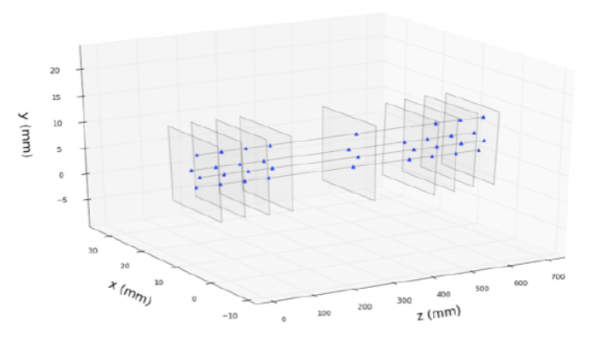
\includegraphics[scale=0.9]{figures/telescope_tracks.png}
\caption{Four example tracks reconstructed in the Timepix3 telescope. Figure taken from \cite{Sophie}.}
\label{fig:telescope_tracks}
\end{figure}


\section{Testbeam measurements}

\subsection{Experimental setup}


\section{Charge sharing}


